\documentclass[a4,11pt]{article}

\usepackage{graphicx}
\usepackage{tabularx}
\usepackage{geometry}

\geometry {
  a4paper,
  top=15mm,
  left=18mm,
  right=18mm,
  bottom=25mm,
}

\usepackage{fontspec}

%-----------------------------------------------------------
% Comment the following lines if Adobe Garamond Pro font is
% not available as `AGaramondPro'
\setmainfont{AGaramondPro}[
  UprightFont   = *-Regular,
  ItalicFont    = *-Italic,
  BoldFont      = *-Semibold,
  BoldItalicFont= *-BoldItalic
]
%-----------------------------------------------------------

\title{OS architecture (OS layers) of Unix, Linux and Windows}
\author{Suyash Mahar \\
  ECE - 16116069
}

\date{\today}

\usepackage{multicol}
\begin{document}

\maketitle


\section{Introduction}
Both Windows and Linux/Unix have similar OS architecture except for a
few differences in the design.

\section{Linux/Unix Kernel}
Linux/Unix are monolithic kernels, which means that they are
implemented as a single codebase with you protection between them. The
kernel however allows small modularity by loading modules in the
kernel. These modules are called Dynamically Loadable Kernel Module
(DLKM). Major layers in the Linux/Unix based operating systems are:

\begin{enumerate}
\item Applications
  \begin{enumerate}
  \item Libraries
  \item System Daemon
  \item Shells
  \item Tools
  \end{enumerate}
\item Operating System
\item Kernel
\item Hardware
\end{enumerate}

\begin{figure}[!ht]
  \centering
  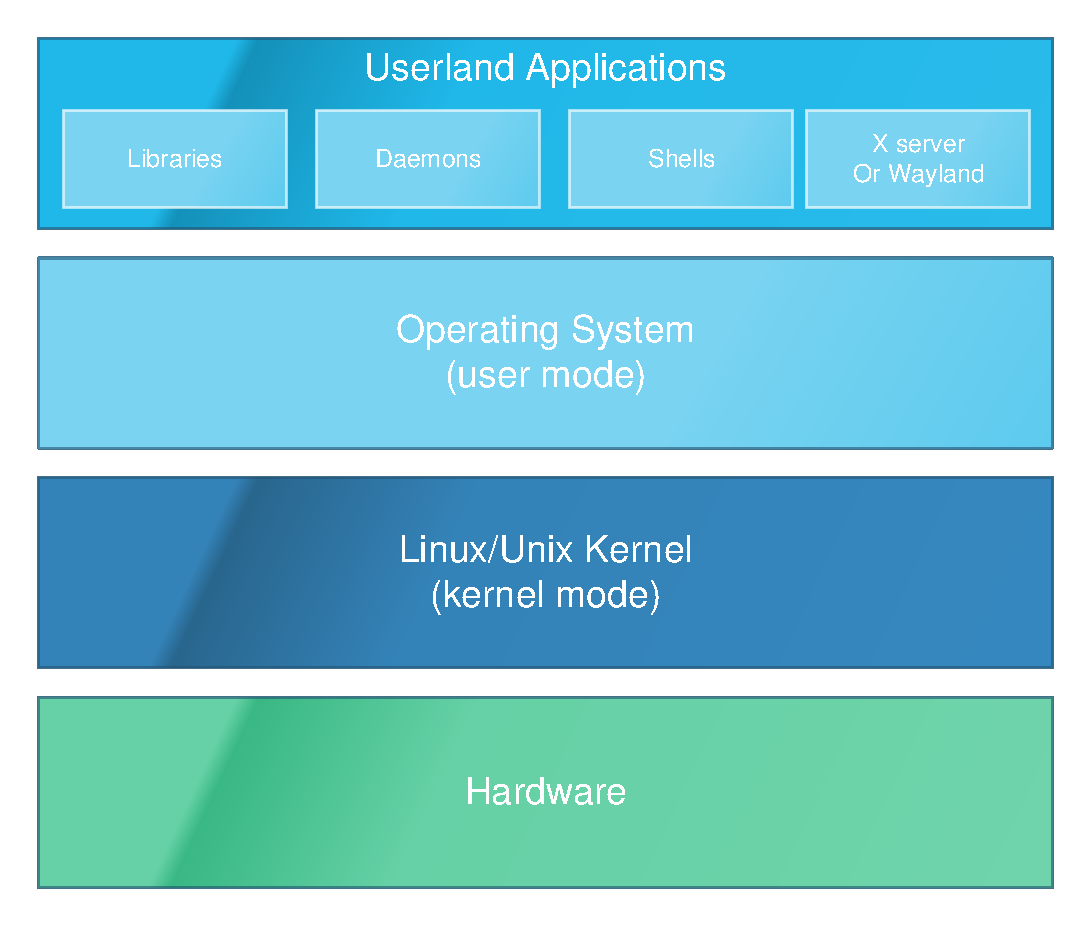
\includegraphics[width=0.5\linewidth]{images/linux-layers.pdf}
  \caption{Linux layered architecture}
  \label{fig:linux-layered}
\end{figure}

\subsection{Approach to Windowing}
Linux/Unix uses X server in user mode to draw graphics, this allows
decoupling graphics subsystem from the kernel. Also, allowing x server
to run in user mode prevents X server errors to de-stabilize the
complete OS.
\section{Windows NT Kernel}

\begin{enumerate}
\item Applications
  \begin{enumerate}
  \item Win32 applications
  \item POSIX compatibility layer
  \item OS/2
  \item Windows Services
  \end{enumerate}
\item Operating System
\item Kernel
  \begin{enumerate}
  \item Kernel level drivers
  \item Display system
  \end{enumerate}
\item Hardware abstration layer
\item Hardware
\end{enumerate}

\begin{figure}[!ht]
  \centering
  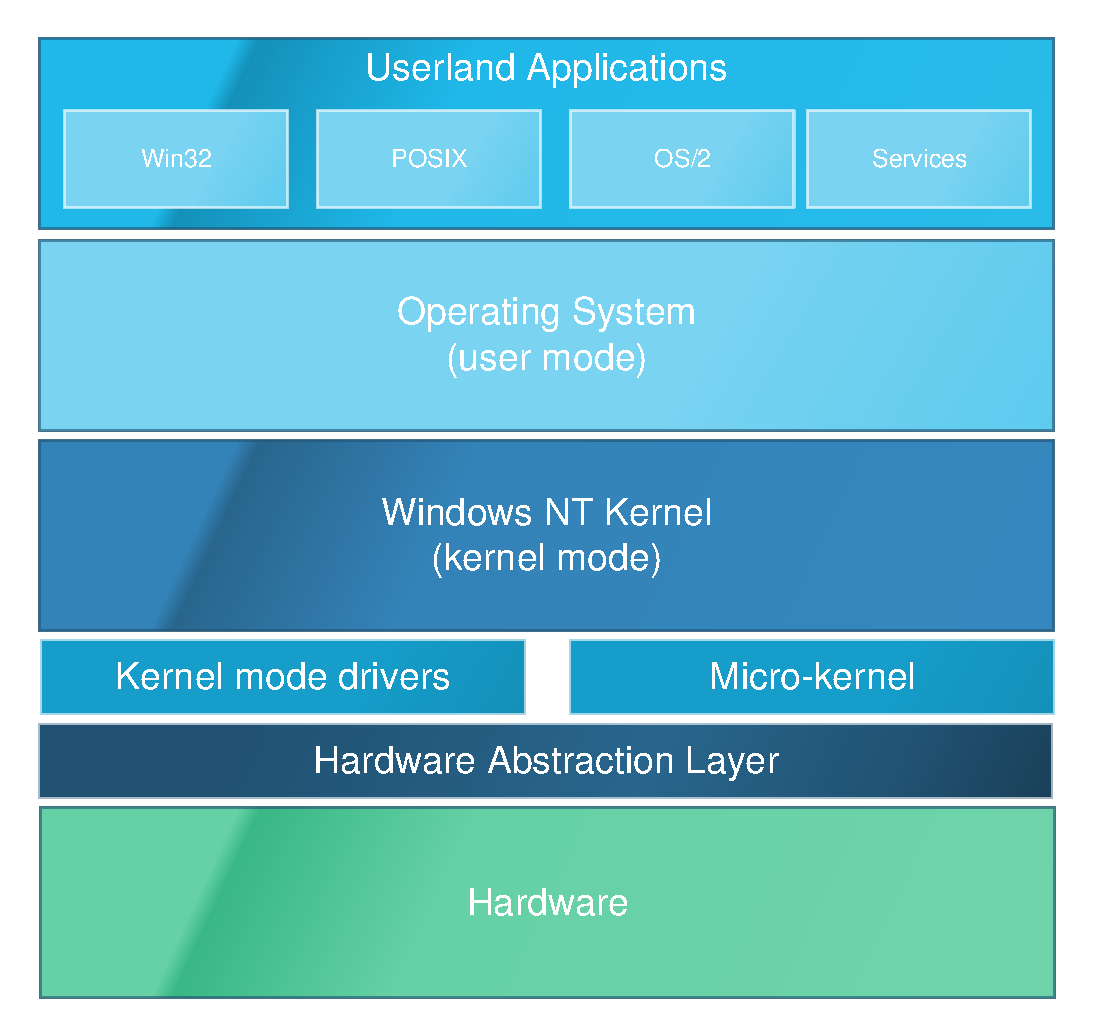
\includegraphics[width=0.5\linewidth]{images/win-nt-layers.pdf}
  \caption{Windows NT layered architecture}
  \label{fig:win-nt-layered}
\end{figure}

\subsection{Approach to Windowing}
Windows Operating System runs its graphics system in kernel mode, this
allows much higher performance then running it in user mode by
avoiding several context switches. Running graphics system in kernel
mode however poses stability and security risks.

\end{document}
